%************************************************
\chapter{The LUX Detector}

\label{ch:LUX} % $\mathbb{ZNR}$
%************************************************

\section{LUX Overview}
The \ac{LUX} detector was an ultra-low background dual-phase liquid xenon \ac{TPC} that set world-leading limits on \ac{WIMP} interactions.
 
\ac{LUX} began underground commissioning in July 2012, moving to the 4850 level (4300~m.w.e) of \ac{SURF} in Lead, South Dakota.  The \ac{LUX} Collaboration's first \ac{WIMP} search exposure was for a period of 85.3 live-days, acquired between April 2013 and August 2013. This period of time is referred to as Run03, and the \ac{WIMP} result is referred to as WS2013. The detector then underwent a grid conditioning campaign to improve voltage capabilities, followed by a series of extensive calibrations to characterize the new operating conditions. The detector then ran for a period of 332 live-days from September 2014 to May 2016 (Run04, WS2014-2016), ending with decommissioning in September 2016. Run03 and Run04 had distinct operating conditions and calibrations. The \ac{LIP} search in Chapter~\ref{ch:lips} was carried out using Run03 data, and the calibrations in the latter half of this chapter describe the detector conditions as they were in Run03. 

\section{Internal Components}
The active volume of \ac{LUX} was composed of 300~kg of liquid xenon, instrumented with two arrays of Hamamatsu R8778 \ac{VUV}-sensitive \ac{PMT}s viewing the liquid region from the top and bottom. Both arrays were composed of 61 \ac{PMT}s that detected S1 and S2 photons from particle interactions in the active liquid volume, and were held in place by copper mounting blocks. The \ac{PMT}s were tightly packed in a hexagonal formation to maximize light collection. The xenon-facing surfaces the of copper \ac{PMT} mounting blocks were covered with \ac{PTFE} tri-foils to reflect the 178~nm light, since copper is a poor reflector of \ac{VUV} light. 

The active region was defined by a series of strung wire or mesh grids: the cathode grid was at the bottom of the detector, and the gate grid was 48.3~cm above the cathode when cold. These two grids formed the drift field, which was \~180~kV/cm during Run03. The region is known as the drift region, it is where particle interactions The anode mesh plane was 1~cm above the gate grid, and the xenon liquid level was held constant between these two electrodes by a spillover weir. The anode and gate form the extraction region of the experiment, where electrons are extracted across the liquid-gas boundary and undergo proportional scintillation to form S2. There are two additional grids, the top and bottom grids, which are placed 2~cm from the top and bottom \ac{PMT} arrays to insulate the \ac{PMT}s from the high fields produced by the other grids. The top and bottom grids were held at approximately the same voltage applied to the \ac{PMT}s. All electrodes were 88\%-99\% optically transparent at normal incidence, and made of stainless steel 316. The major components of \ac{LUX} are shown in Figure~\ref{fig:lux1}

\begin{figure}[htbp]
\begin{center}
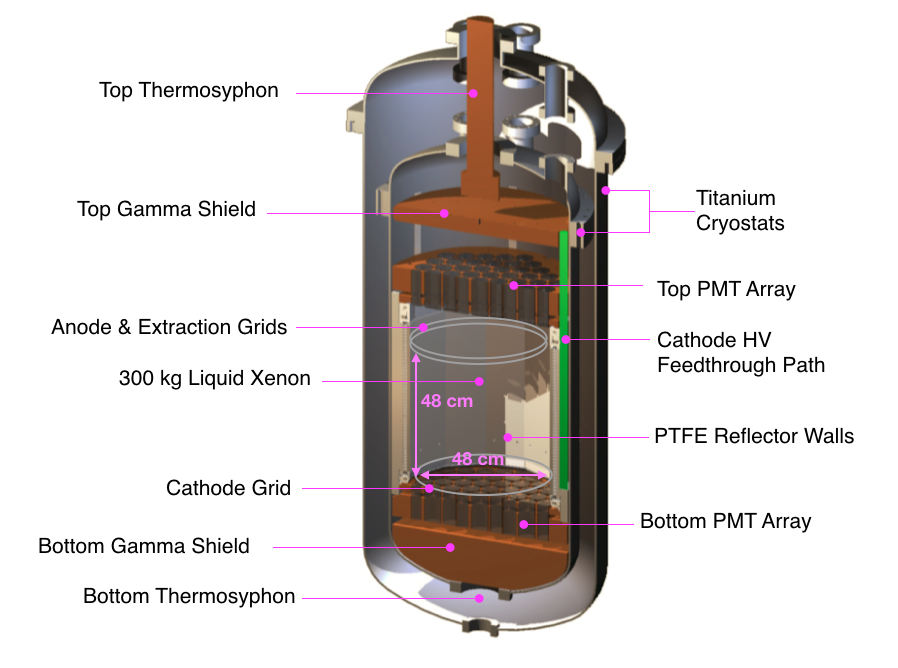
\includegraphics[width=\textwidth]{figures/lux/lux_inner1.png}
\caption{Major components and dimensions of the LUX detector.}
\label{fig:lux1}
\end{center}
\end{figure}


The insides of the detector walls were lined with 12 \ac{PTFE} panels, which made the exact detector geometry a dodecagonal prism with flat faces, instead of a cylinder one rounded face. Immediately behind the \ac{PTFE} were 48 copper field-shaping ``rings'' (dodecagons). The rings were vertically separated by 1~cm, and the gate-to-cathode voltage was graded evenly over the rings by a resistor chain connecting the rings. 

Below and above the \ac{PMT} mounting blocks were two large solid copper domes which act as gamma shields and also function as thermal mass that aid in keeping the detector temperature stable. The bottom dome also acts as a heat exchanger to quickly re-thermalize incoming xenon gas (from the circulation system) as it enters the liquid region, and minimizes the volume filled with non-active liquid xenon. See Figure~\ref{fig:lux2} for details of the field-shaping rings and copper shields.

\begin{figure}[htbp]
\begin{center}
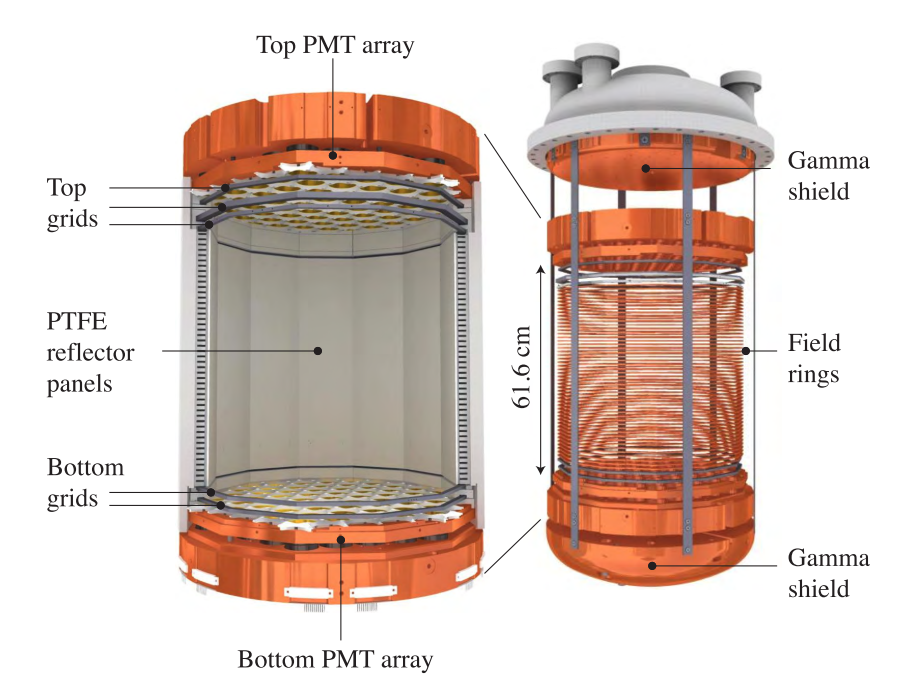
\includegraphics[width=\textwidth]{figures/lux/lux_inner2.png}
\caption{Field-shaping rings detail}
\label{fig:lux2}
\end{center}
\end{figure}


More details about the internal components can be found in C. Faham's PhD thesis \cite{Faham2014a}.

\section{External Components}

The \ac{LUX} cryogenic system was based on thermosyphons, which deliver ``cooling power'' to solid copper cold heads, which are in thermal contact with the liquid xenon space. A simplified diagram is shown in Figure~\ref{fig:luxcryo}. A thermosyphon is a closed-loop cooling device containing a thermal messenger gas; N$_{2}$ is a common choice and was the choice for the \ac{LUX} thermosyphons. The top of the thermosyphon is immersed in a bath of liquid nitrogen, and the bottom is in thermal contact with the liquid xenon space. The internal messenger gas condenses at the top and drips down to the cold head, where it absorbs heat from the xenon space, evaporates, and returns to the top of the thermosyphon to condense and repeat the cycle. In this manner, heat from the liquid xenon space is transferred to the external nitrogen bath, which boils off and must be periodically replenished. The pressure of the internal nitrogen messenger gas can be adjusted, providing more or less cooling power as desired. The \ac{LUX} thermosyphons were also instrumented with resistive heaters, for further fine control. Four thermosyphons were used to operate the \ac{LUX} detector stably at \~175~K with a xenon vapor pressure of \~2~bar. 

\begin{figure}[htbp]
\begin{center}
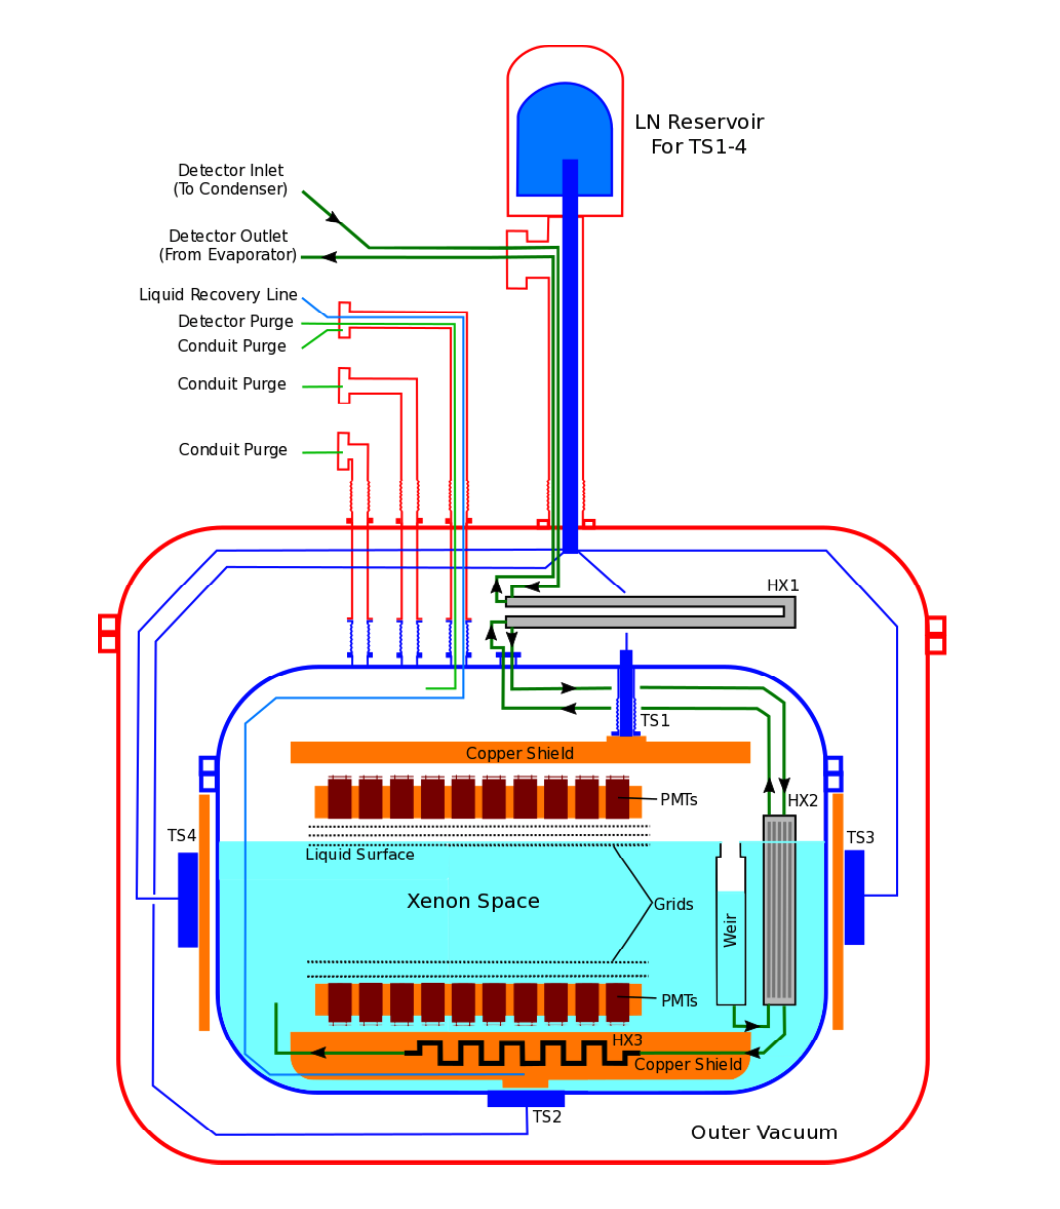
\includegraphics[width=\textwidth]{figures/lux/lux_cryostats.png}
\caption{A simplified diagram of the LUX cryogenic system. \cite{NicolesThesis}}
\label{fig:luxcryo}
\end{center}
\end{figure}

The spillover liquid xenon from the liquid-level-setting weir mentioned above was directed into a circulation system through a series of heat exchangers that helped thermalize clean, incoming xenon gas. The xenon circulation was driven by one twin-head KNF double-diaphragm pump, which pushed dirty xenon from the spillover weir through a SAES MonoTorr heated zirconium getter to remove non-noble impurities before returning the clean xenon gas into the detector. A sampling system was able to pull xenon gas samples from different parts of the circulation system and measure impurity content, as well as test for the presence of $^{85}$Kr \cite{Dobi2011}, a troublesome beta emitter which must be removed from the xenon prior to carrying out a successful \ac{WIMP} search.

The circulation pump was installed in parallel with a backup pump, which could be switched on immediately in case of a pump outage. Flow was regulated to the system by two high-flow Brooks \ac{MFC}s. Additional low-flow \ac{MFC}s controlled purge flow through the cabling conduits in Figure~\ref{fig:luxcryo} to ensure gas flow was away from the detector and prevent any contaminants from diffusing into the active xenon space.

Internal calibration sources were plumbed in to alternate flow paths of the circulation system. Xenon gas could be directed through a substrate source, such as the $^{83m}$Kr source described below, to pull $^{83m}$Kr into the detector volume. A bottle containing a source such as the CH$_{3}$T source described below, could be used to deposit the gaseous source in an evacuated section of pipe. Xenon could then be directed through the section of pipe containing the source, to sweep it into the detector volume. 

Lastly, \ac{LUX} was placed in a 7.6~m diameter, 6.1~m high water tank (Figure~\ref{fig:luxwatertank}). The shielding provided by the water tank attenuated the $\gamma$ background from the cavern walls and thermalized neutrons from cavern background radioactivity and muon spallation neutrons. The water tank provided superior shielding from cavern radioactivity such that the detector backgrounds were dominated by the radioactivity of internal detector components, which in turn were controlled through a strict campaign of cleanliness and choice of detector materials \cite{LUXDetectorPaper}, \cite{LUXRun03Backgrounds}. Vertical tubes visible in Figure~\ref{fig:luxwatertank} were used to deploy external calibration sources at different heights, such as $^{137}$Cs, which were directed into the detector via a collimating source assembly.


\begin{figure}[htbp]
\begin{center}
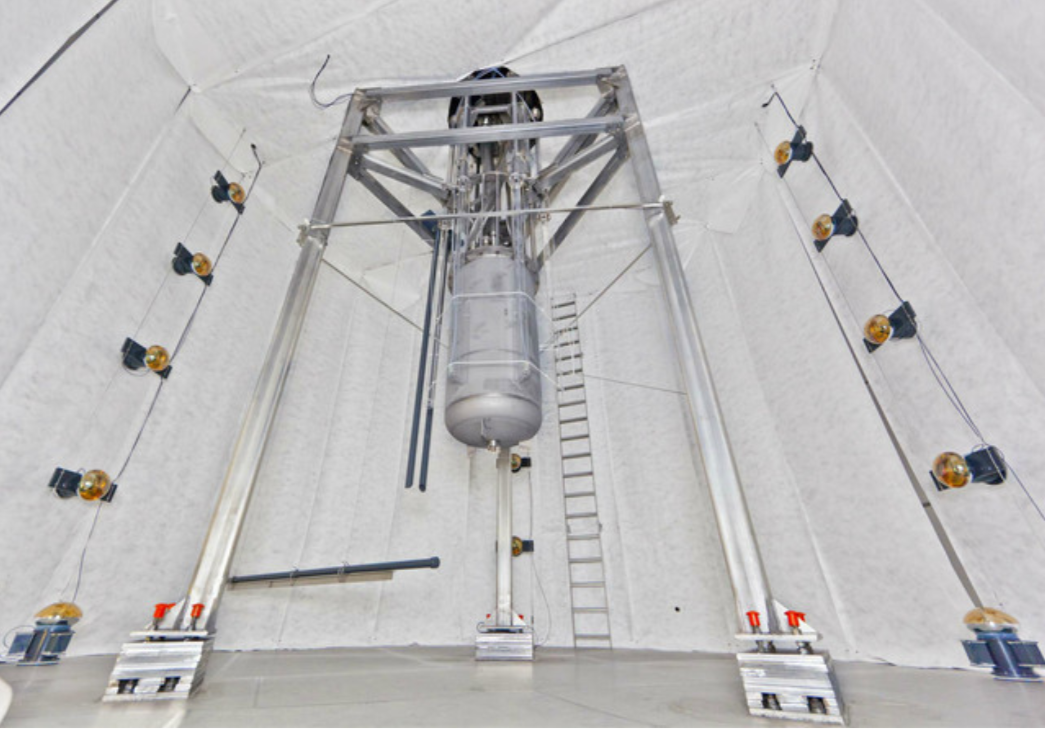
\includegraphics[width=\textwidth]{figures/lux/lux_watertank.png}
\caption{A photo of the LUX detector installed inside the water tank.}
\label{fig:luxwatertank}
\end{center}
\end{figure}

The \ac{LUX} detector water tank and material screening achieved the low background in the \ac{WIMP} search energy range shown in Figure~\ref{fig:luxrun03bkg}

\begin{figure}[htbp]
\begin{center}
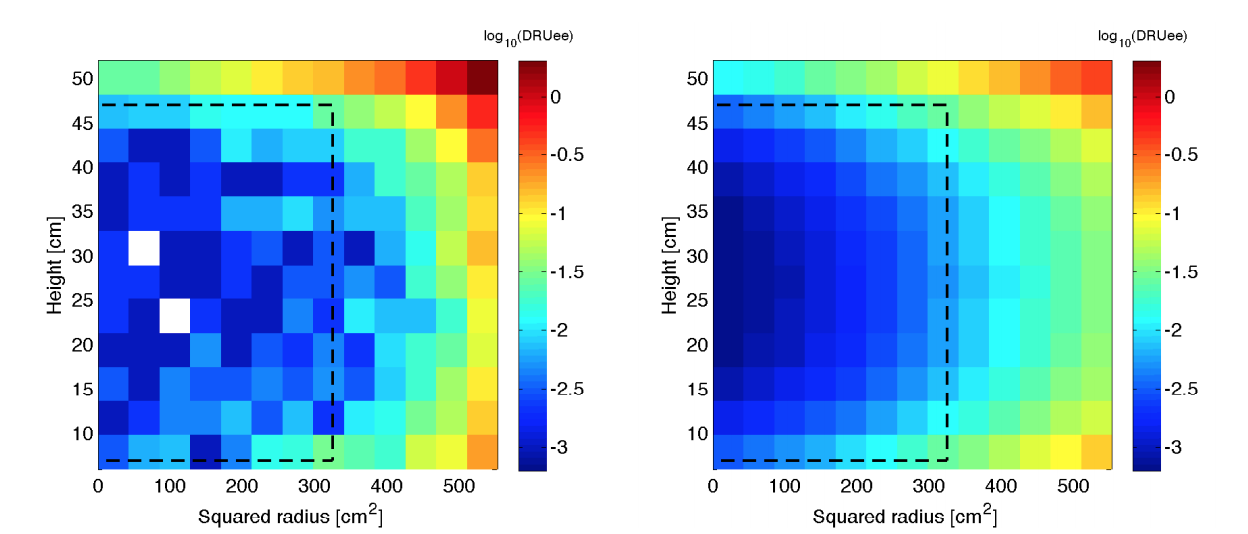
\includegraphics[width=\textwidth]{figures/lux/lux_run03bkg.png}
\caption{Backgrounds distributions in squared radius and height for expected (right) and measured (left) backgrounds in the energy range 0.9-5.3~keV$_{ee}$ (2-30 phe S1) for the 85.3 live-day Run03 \ac{WIMP} exposure. Black lines show the 118~kg fiducial mass. Units are log$_{10}$DRU$_{ee}$, electron equivalent differential rate units, i.e. keV$_{ee}^{-1}$kg$^{-1}$day$^{-1}$.  Figure from \cite{LUXRun03Backgrounds}. }
\label{fig:luxrun03bkg}
\end{center}
\end{figure}


\section{Trigger and Data Acquisition}
Cabling for PMTs and other monitoring instrumentation were routed from the inner detector volume to the outside via conduits illustrated in in Figure~\ref{fig:luxcryo}. The \ac{PMT} signals are amplified Figure~\ref{fig:luxdaq}

\begin{figure}[htbp]
\begin{center}
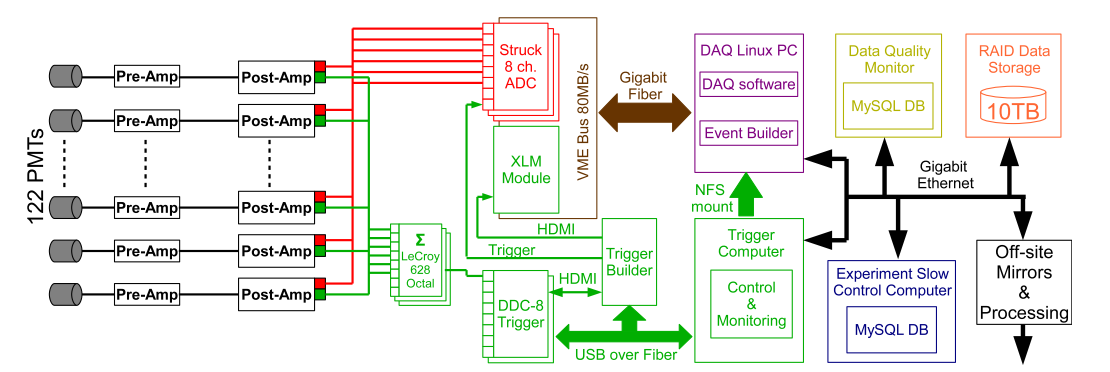
\includegraphics[width=\textwidth]{figures/lux/lux_daq.png}
\caption{Overview of the LUX trigger system. Figure from \cite{LUXTrigger}. }
\label{fig:luxdaq}
\end{center}
\end{figure}


\section{Data Processing}


\section{Calibrations}
\subsection{Energy}
Recall from Section~\ref{sec:energy_reconstruction} that the electron-equivalent energy of an event in a dual phase xenon \ac{TPC} is reconstructed as follows:

\begin{equation}
E = W (\frac{S1}{g_{1}} + \frac{S2}{g_{2}})
\end{equation}

 
Two or more calibration line sources of different energies are required to fit for the detector gains $g_{1}$ and $g_{2}$. The \ac{LUX} experiment uses a suite of sources to calibrate the energy response of the detector, shown in \ref{fig:calib_sources}.

\begin{figure}[htbp]
\begin{center}
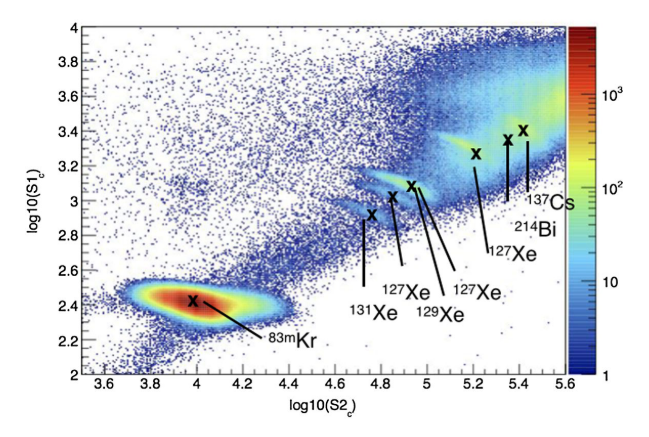
\includegraphics[width=\halffig]{figures/lux/calibration_sources.png}
\caption{Plot showing calibration sources (Figure from \cite{LUX:Run03Comprehensive}. The axis label subscript $c$ denotes corrected variables with calibration for geometrical effects and electron lifetime (these corrections are discussed in Section~\ref{sec:krypton}.}
\label{fig:calib_sources}
\end{center}
\end{figure}

The average S1 and S2 of each calibration source is normalized to the true energy:

\begin{equation}
(S1, S2) \longrightarrow \Big(\frac{\langle S1 \rangle}{E}, \frac{\langle S2 \rangle}{E}\Big)
\end{equation}

and a line $y = mx + b$ is fit to the transformed variables, where the slope is $m = -g_{1} / g_{2}$ and the y-intercept is $b = g_{1} / W$. 

\begin{figure}[htbp]
\begin{center}
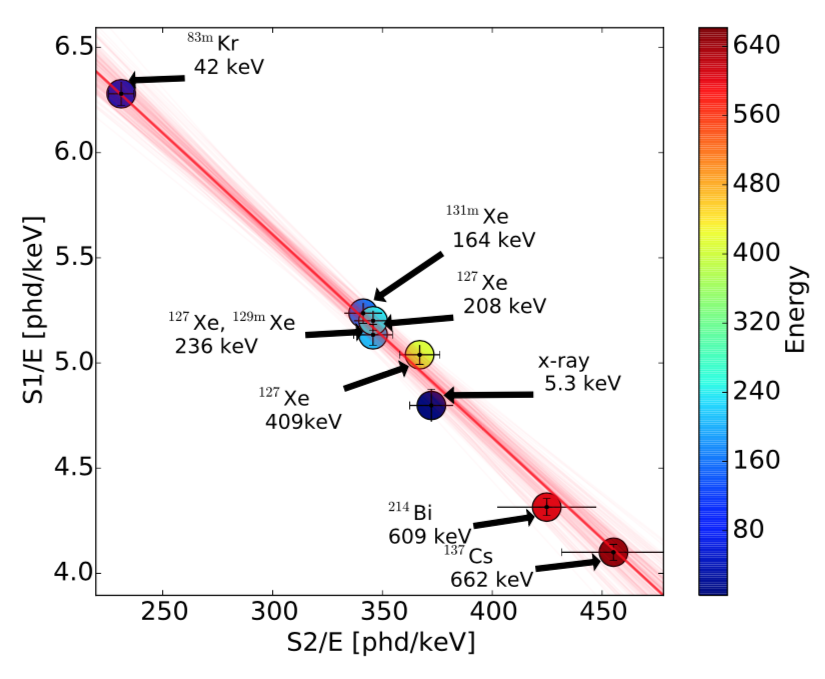
\includegraphics[width=\halffig]{figures/lux/doke.png}
\caption{ Doke plot used to fit $g_{1}$ and $g_{2}$ for LUX Run03 (Figure from \cite{LUX:Run03Comprehensive}}
\label{fig:doke}
\end{center}
\end{figure}

From the fit in Figure~\ref{fig:doke}, the \ac{LUX} gains for Run03 were measured to be $g_{1} = 0.117 \pm 0.003$~phd/photon and $g_{2} = 12.1 \pm 0.8$~phd/electron. Single electrons are periodically emitted into the gas and undergo proportional scintillation. This phenomenon is well known in liquid xenon detectors and is discussed further in Chapter~\ref{ch:etrains}. A sample of pure single electrons was collected to find the average number of S2 photons produced by one electron, referred to the single electron size. The single electron size in Run03 was a skew-gaussian with mean 24.66 phd and a 1-$\sigma$ width of 5.95 phd. Combing this with $g_{2}$ gives an \ac{EEE} of $49\% \pm 3\%$ \cite{LUX:Run03Comprehensive}.


\subsection{Tritium - ER Band and Yields}


\subsection{DD - NR Band and Yields}


\subsection{Kr - Geometrical Light Collection Corrections}
\label{sec:krypton}




%*****************************************
%*****************************************
%*****************************************
%*****************************************
%*****************************************
